\documentclass[12pt, a4paper, oneside, fontset=windows]{ctexbook}
\usepackage{amsmath, amsthm, amssymb, bm, graphicx, hyperref, mathrsfs}
% 让图像路径兼容从仓库根目录编译
\graphicspath{{./一维随机游动/}{./}}
\usepackage{tcolorbox}
\usepackage{tikz}
\usetikzlibrary{tikzmark, arrows.meta, shapes}
\usepackage{geometry}
\geometry{a4paper, margin=1in}
\setlength{\parindent}{0pt}
\setlength{\parskip}{1em}

\title{{\Huge{一维随机游动}}\\课程笔记附录:解题过程图示}
\author{刘明琦}
\date{\today}
\linespread{1.3}

% 定理环境(与仓库统一)
\newtheorem{theorem}{定理}[section]
\newtheorem{definition}{定义}[section]
\newtheorem{lemma}[theorem]{引理}
\newtheorem{corollary}[theorem]{推论}
\newtheorem{example}{例}[section]
\newtheorem{proposition}[theorem]{命题}

% 常用算子(与仓库统一)
\DeclareMathOperator*{\esssup}{ess\,sup}
\DeclareMathOperator{\st}{\mathrm{s.t.}}
\DeclareMathOperator{\diff}{\mathrm{i.f.f.}}
\DeclareMathOperator{\ie}{\mathrm{i.e.}}

\begin{document}

\maketitle

\pagenumbering{roman}
\setcounter{page}{1}
\begin{center}
	\Huge\textbf{前言}
\end{center}~\\
本附件整理了“一维随机游动”问题的解题过程要点,并配套展示了五张过程图示(1.jpg–5.jpg)。为保持与主笔记一致,采用 XeLaTeX 与统一的版式和环境设置。

\begin{flushright}
	\begin{tabular}{c}
		刘明琦\\
			oday
	\end{tabular}
\end{flushright}

\newpage
\pagenumbering{Roman}
\setcounter{page}{1}
	ableofcontents
\newpage
\setcounter{page}{1}
\pagenumbering{arabic}

\chapter{问题与解答概览}

\begin{tcolorbox}
	extbf{问题背景(概述)}\\
考虑一维随机游动:粒子以步长 $\pm 1$(或一般步长)在整数线上移动。典型关注量包括:首次到达某点的概率、预期返回时间、吸收边界下的吸收概率与期望步数、偏置游动的极限行为等。本章仅整理图示步骤,不替代完整推导。
\end{tcolorbox}

\section{解题过程图示}
下列图示按解题顺序排列。若需插入文字注释或推导公式,可在对应图之后添加段落或公式环境。

\begin{figure}[h]
	\centering
	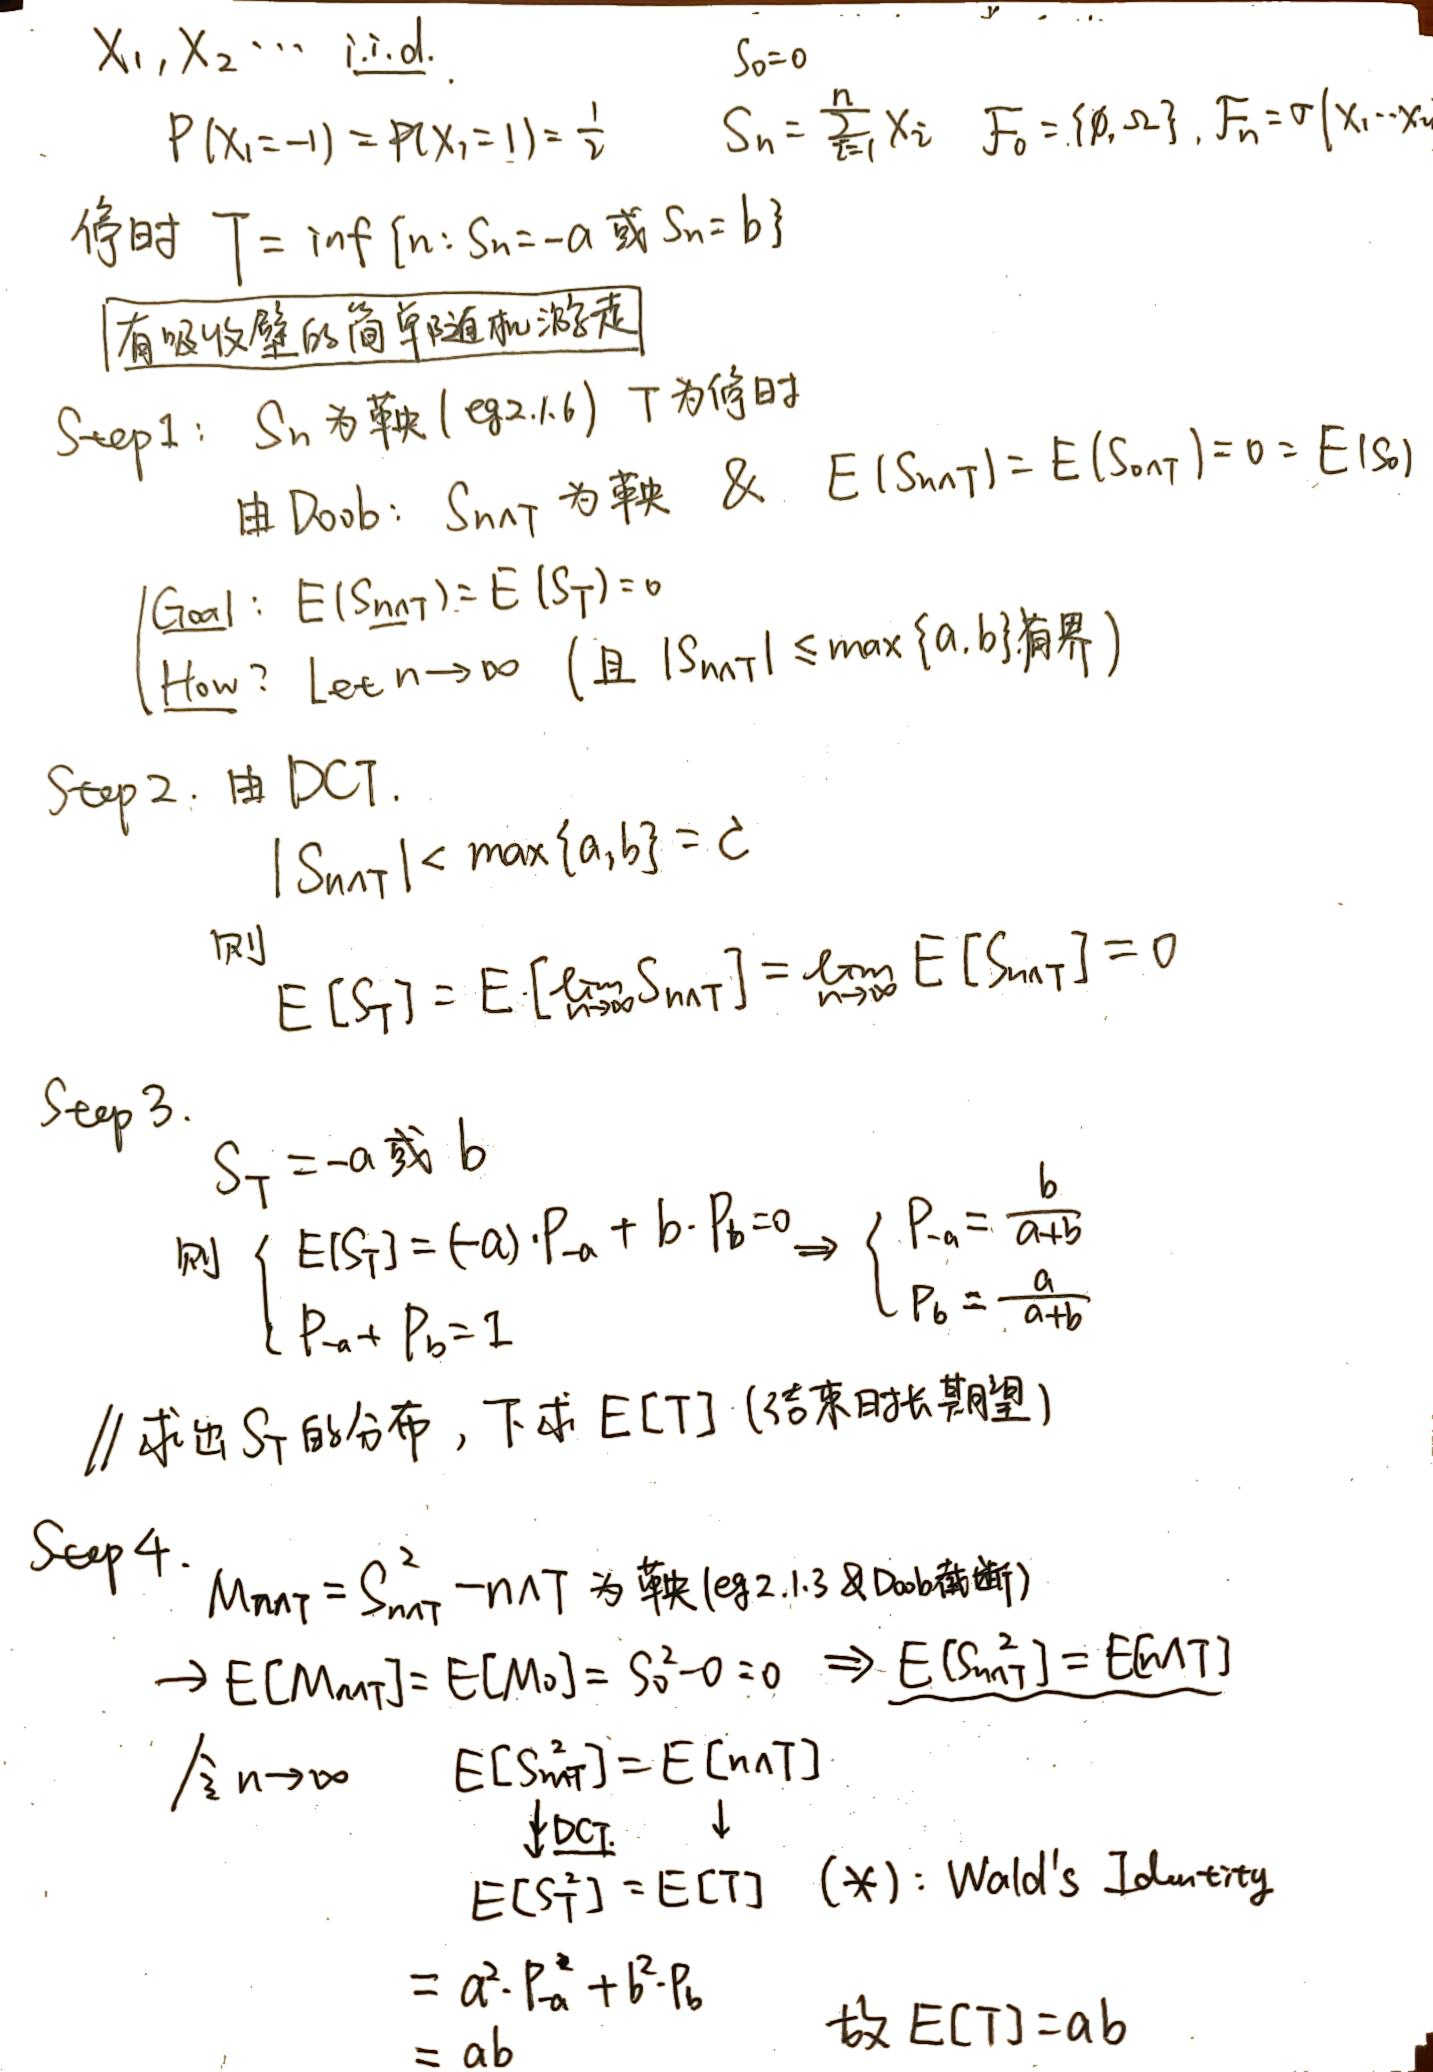
\includegraphics[width=0.92\textwidth]{1.jpg}
	\caption{步骤 1:问题建模与基本设定(示意)}\label{fig:rw-step1}
\end{figure}

\begin{figure}[h]
	\centering
	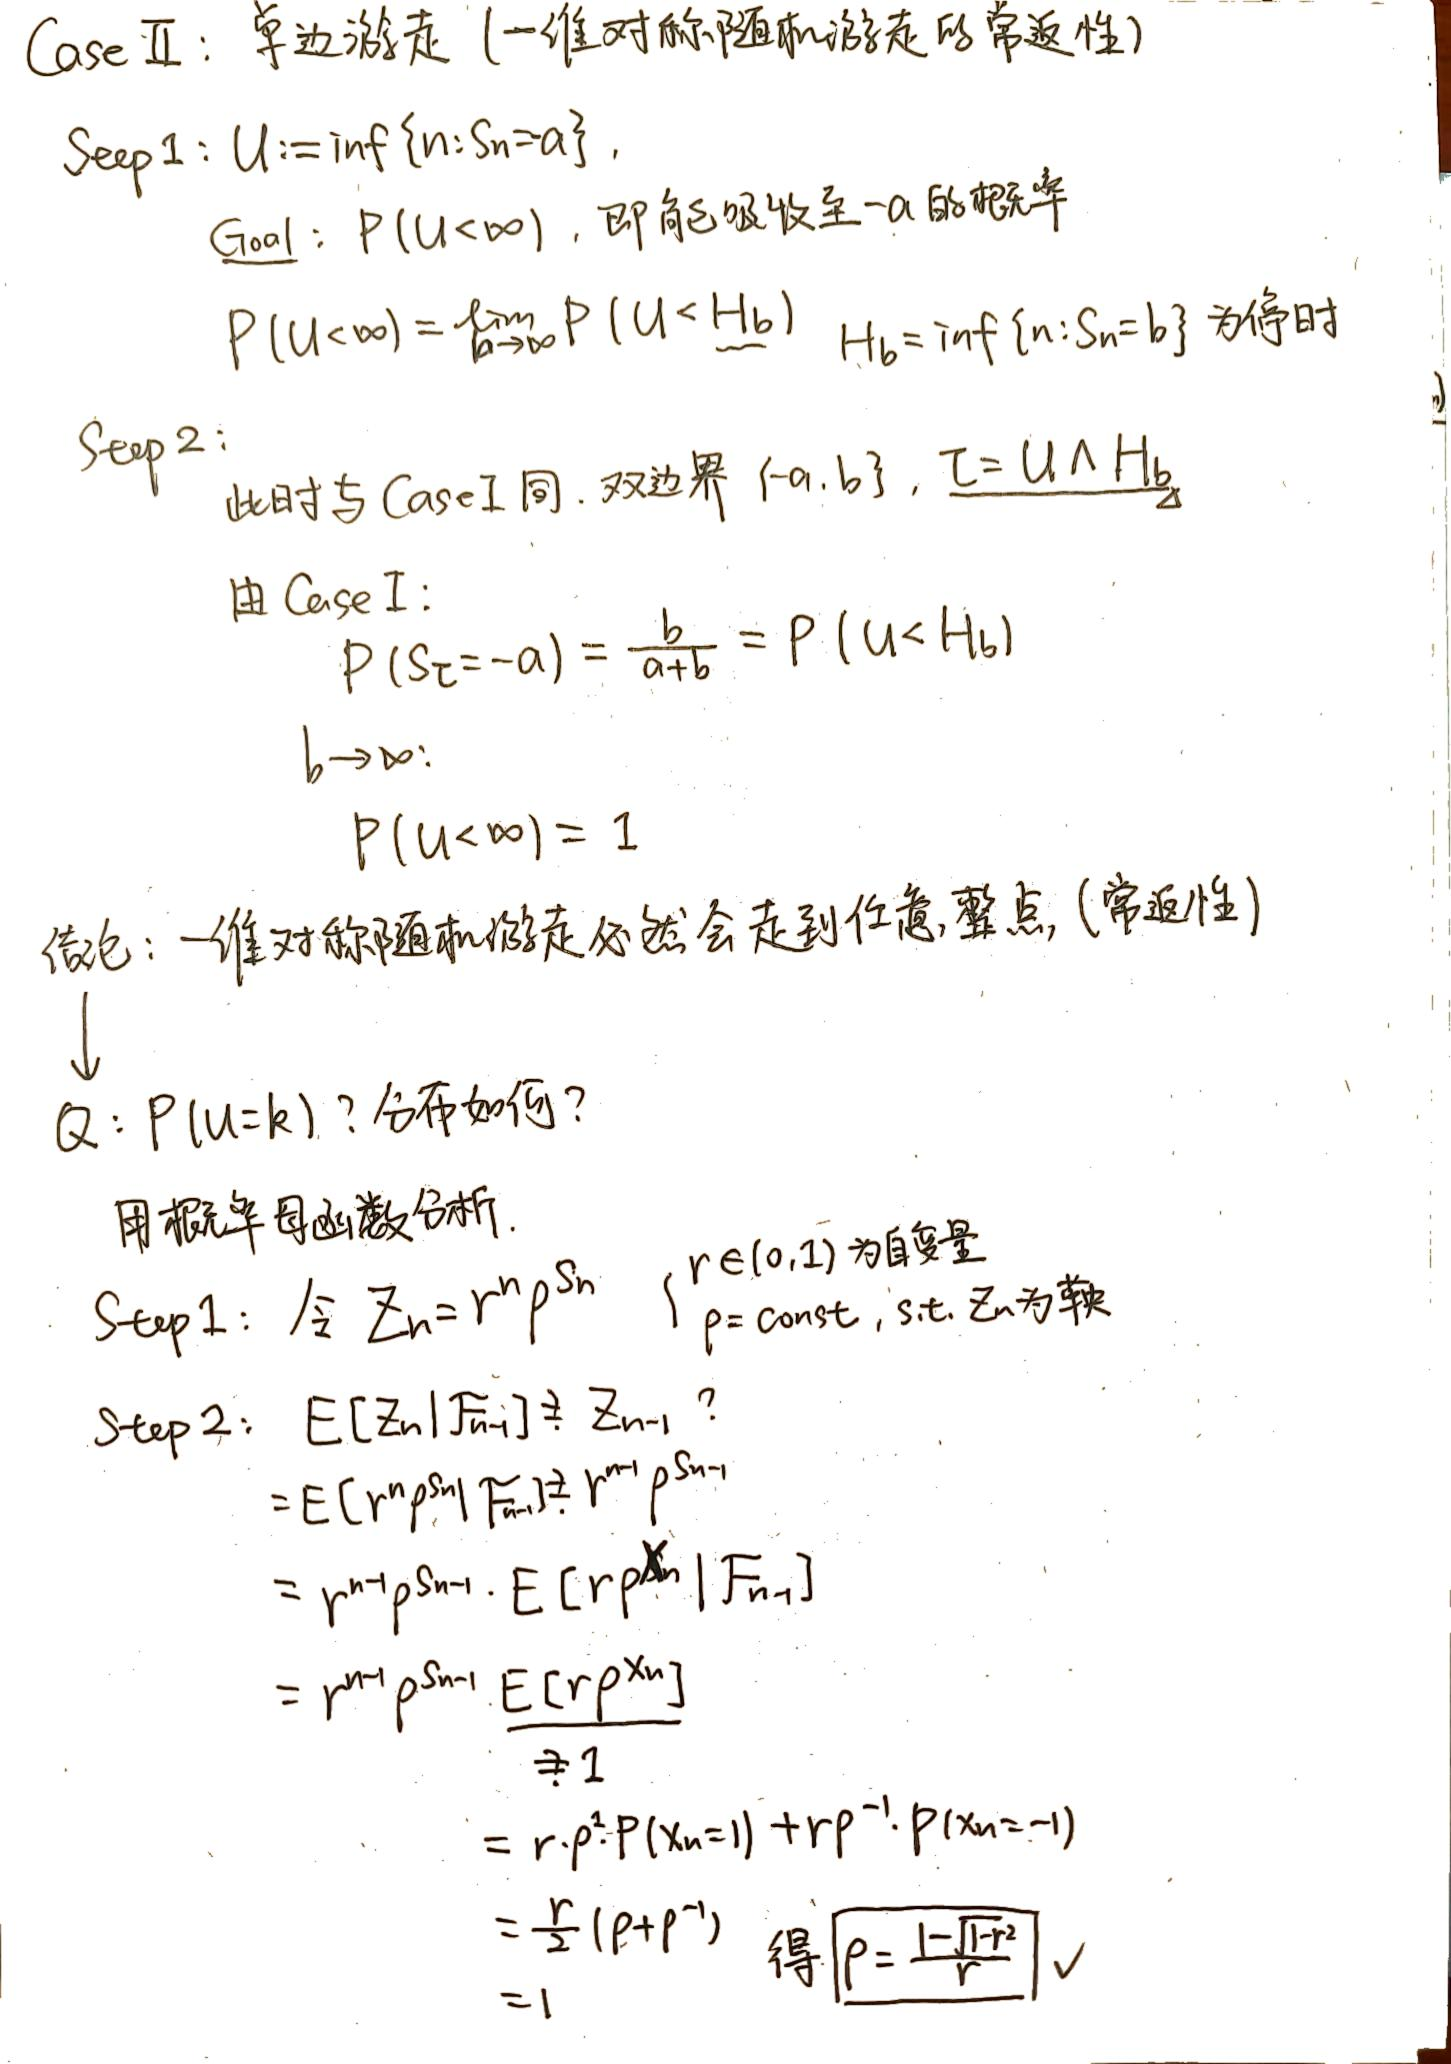
\includegraphics[width=0.92\textwidth]{2.jpg}
	\caption{步骤 2:关键量的递推/差分方程(示意)}\label{fig:rw-step2}
\end{figure}

\begin{figure}[h]
	\centering
	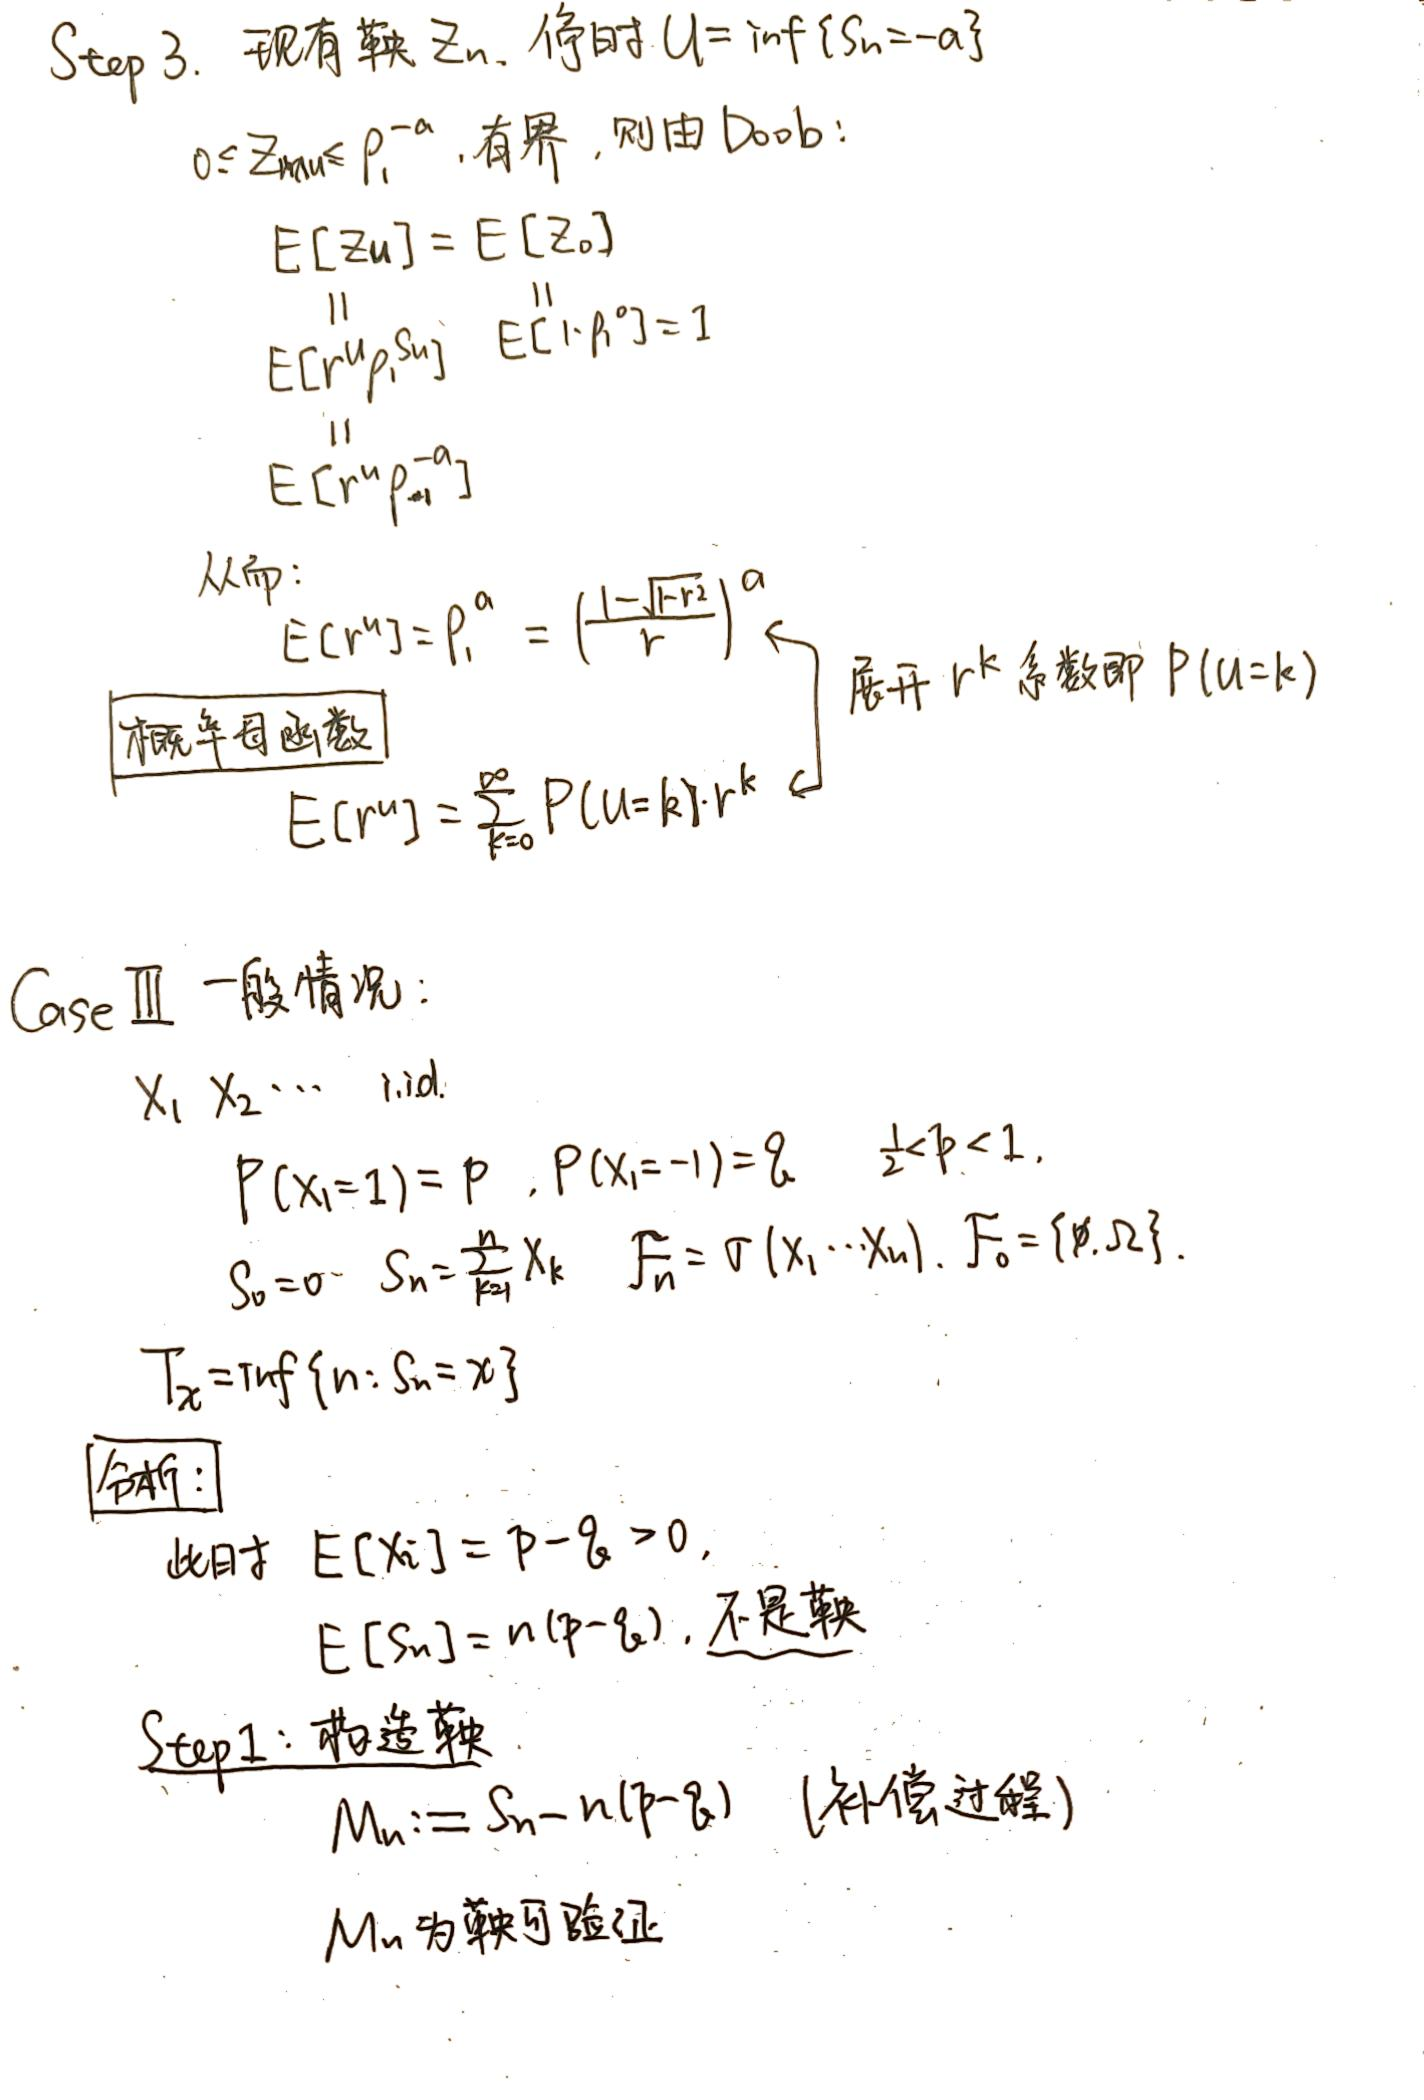
\includegraphics[width=0.92\textwidth]{3.jpg}
	\caption{步骤 3:边界条件与通解结构(示意)}\label{fig:rw-step3}
\end{figure}

\begin{figure}[h]
	\centering
	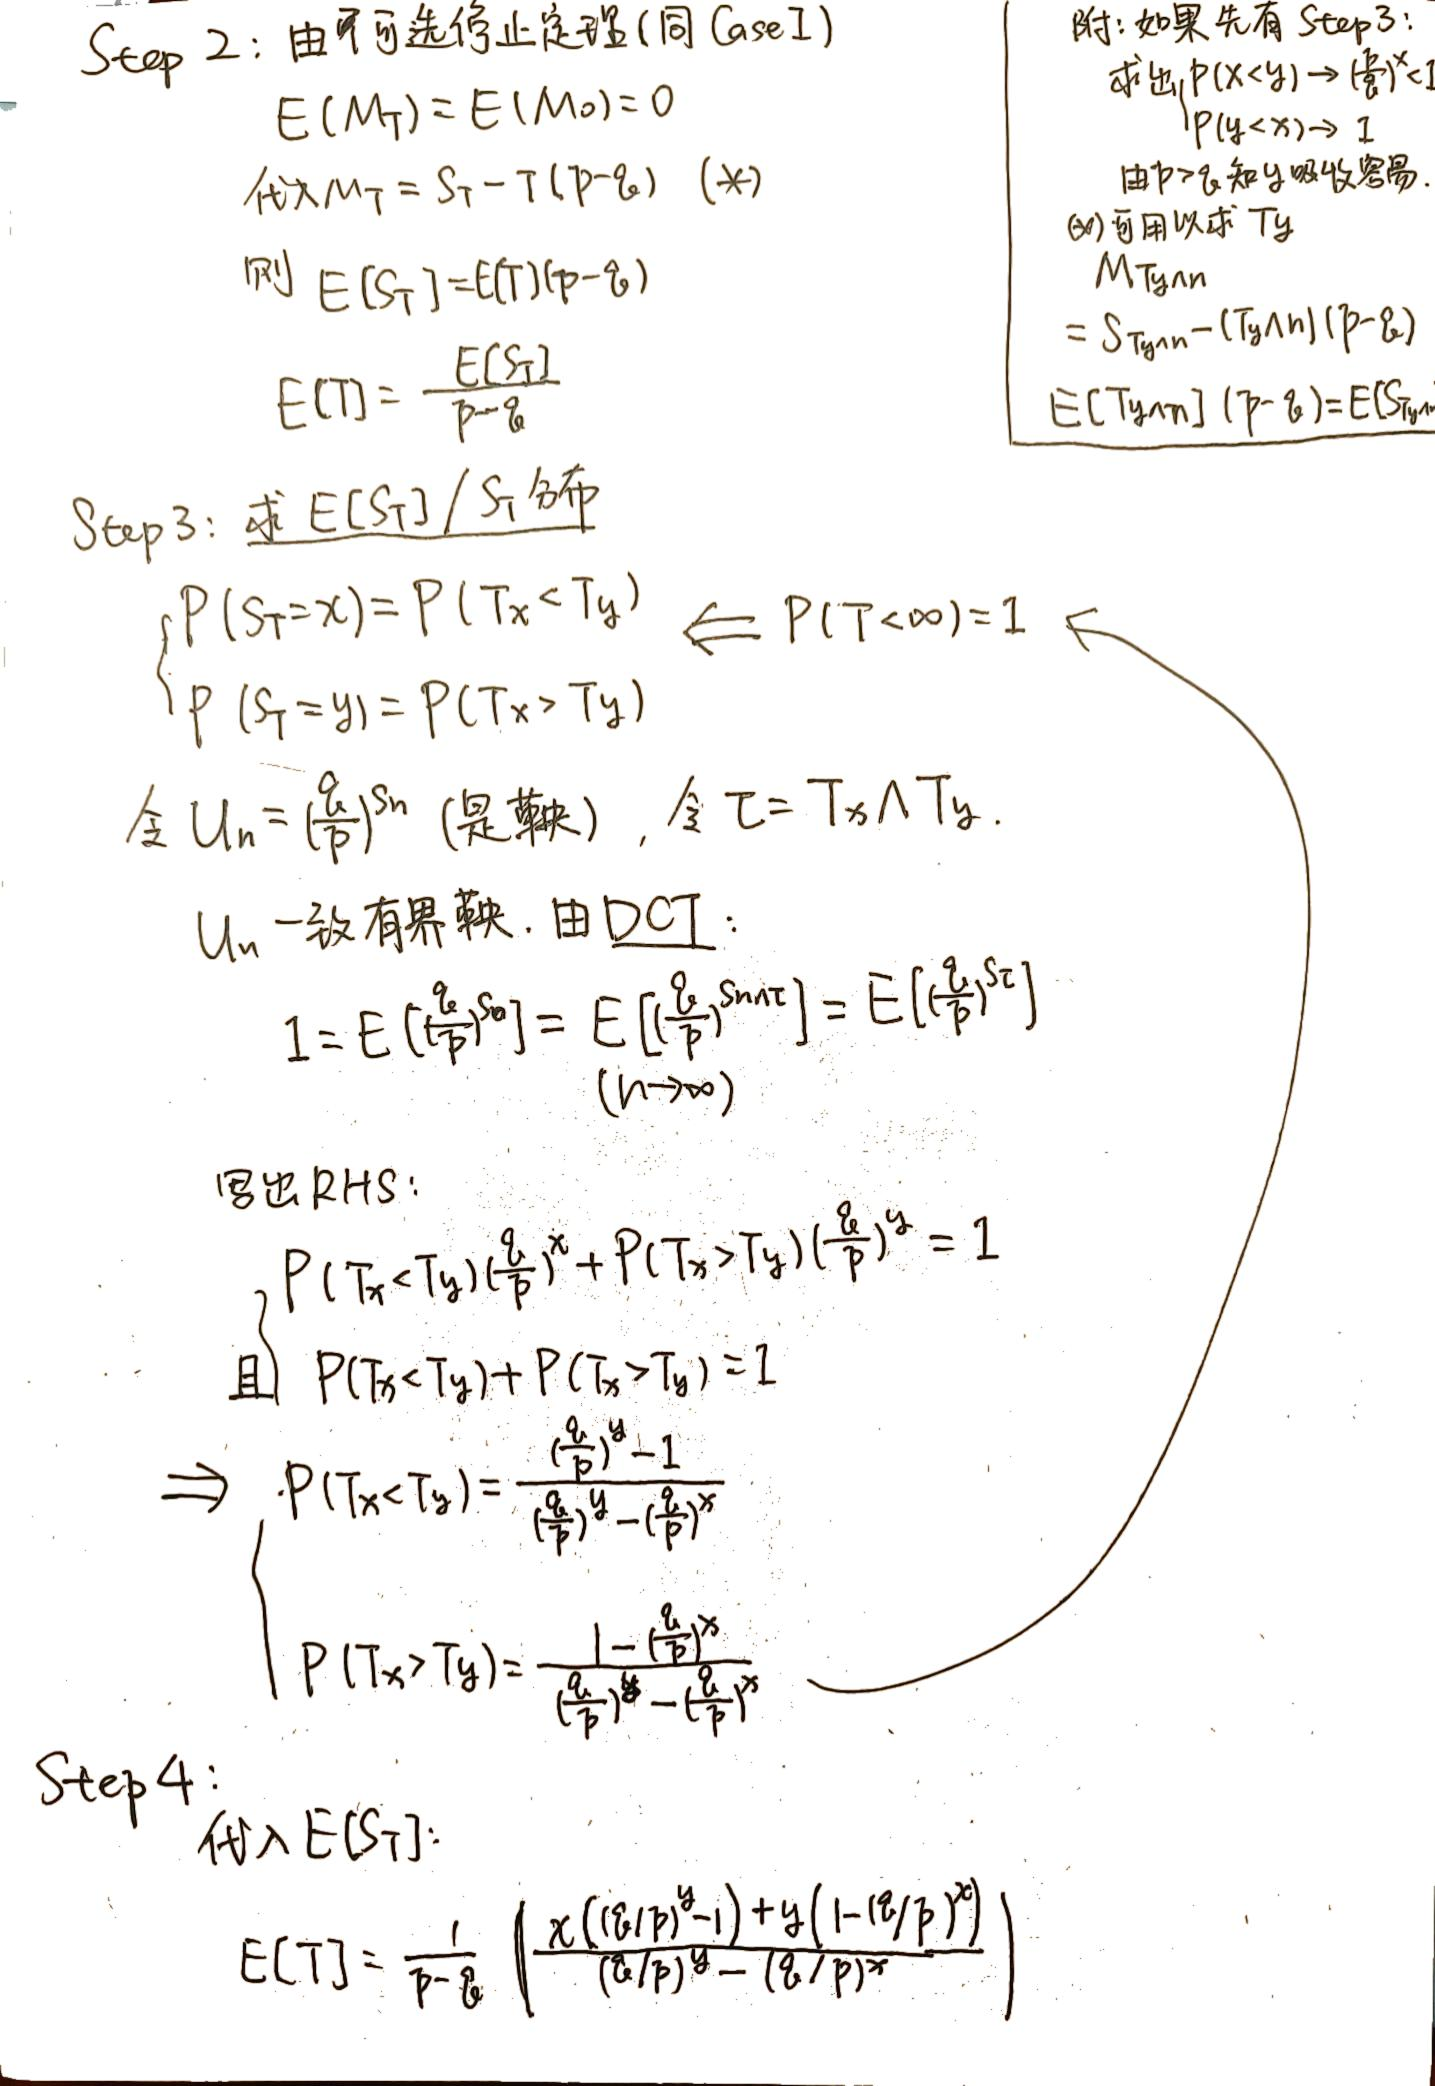
\includegraphics[width=0.92\textwidth]{4.jpg}
	\caption{步骤 4:常数确定与概率/期望解(示意)}\label{fig:rw-step4}
\end{figure}

\begin{figure}[h]
	\centering
	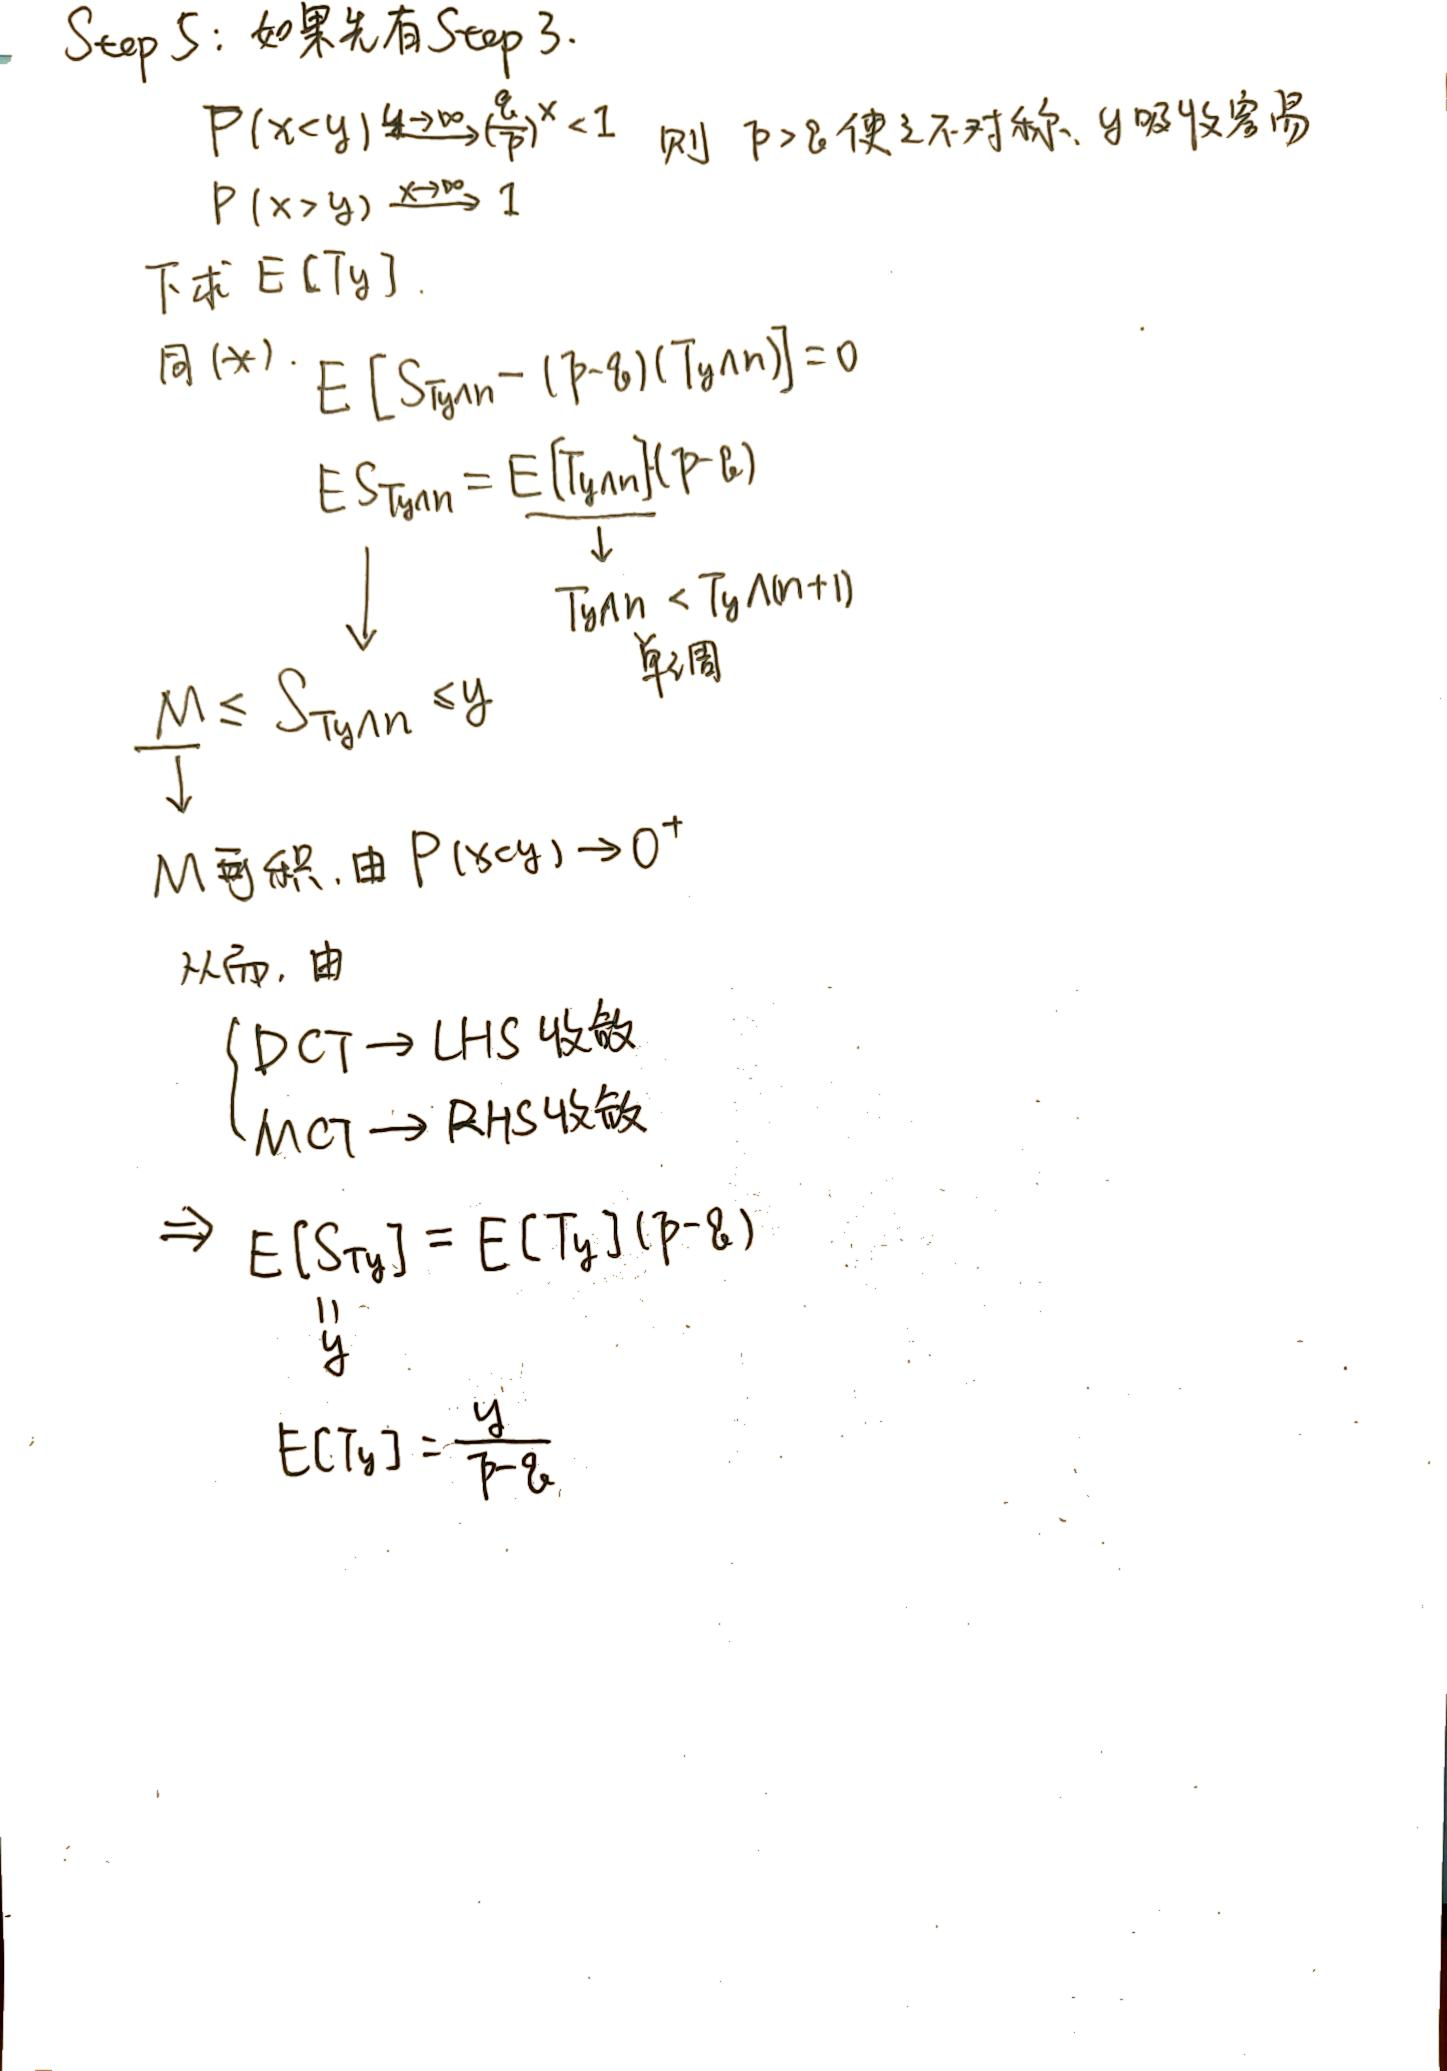
\includegraphics[width=0.92\textwidth]{5.jpg}
	\caption{步骤 5:结论与特殊情形讨论(示意)}\label{fig:rw-step5}
\end{figure}

\vspace{1em}
\noindent
如需将每一步转写为可检验的公式推导,我可以基于你的文字或草图内容补齐相应的差分/边值问题与闭式解,并将证明与说明整理为定理-推论-例题的结构。

\chapter{详细推导过程}
本章将图片中的手写笔记转写为 LaTeX 代码,包含对有界随机游走、常返性以及有偏游走三种情形的详细分析。

\section{Case I:有吸收壁的简单对称随机游走}
\begin{itemize}
    \item 设 $X_1, X_2, \dots$ 独立同分布(i.i.d.),且 $P(X_i=1) = P(X_i=-1) = 1/2$。
    \item 随机游走过程定义为 $S_0=0, S_n = \sum_{i=1}^n X_i$。
    \item 信息流(filtration)为 $\mathcal{F}_n = \sigma(X_1, \dots, X_n)$。
    \item 定义停时 $T = \inf\{n: S_n = -a \text{ or } S_n = b\}$,其中 $a,b > 0$。
\end{itemize}

\subsection{Step 1-3: 计算吸收概率 $P(S_T=-a)$}
\begin{enumerate}
    \item \textbf{构造鞅}: 过程 $S_n$ 是一个鞅,因为 $E[S_n|\mathcal{F}_{n-1}] = S_{n-1} + E[X_n] = S_{n-1}$。
    根据 Doob 可选停止定理,对于停时 $T$,过程 $S_{n \wedge T}$ 也是一个鞅,因此 $E[S_{n \wedge T}] = E[S_0] = 0$。

    \item \textbf{应用控制收敛定理 (DCT)}: 我们的目标是证明 $E[S_T]=0$。
    由于 $S_n$ 在停时 $T$ 之前始终位于 $(-a, b)$ 区间内,所以 $|S_{n \wedge T}| \le \max(a,b)$,即 $S_{n \wedge T}$ 是一致有界的。
    当 $n \to \infty$ 时,$S_{n \wedge T} \to S_T$。根据控制收敛定理,我们可以交换期望和极限:
    \[ E[S_T] = E[\lim_{n \to \infty} S_{n \wedge T}] = \lim_{n \to \infty} E[S_{n \wedge T}] = 0 \]

    \item \textbf{求解吸收概率}: 在停时 $T$ 刻,$S_T$ 的取值只能是 $-a$ 或 $b$。设 $P_a = P(S_T=-a)$ 和 $P_b = P(S_T=b)$。
    我们有两个方程:
    \begin{align*}
        E[S_T] = (-a) \cdot P_a + b \cdot P_b &= 0 \\
        P_a + P_b &= 1
    \end{align*}
    解此方程组可得:
    \[ P(S_T=-a) = \frac{b}{a+b}, \quad P(S_T=b) = \frac{a}{a+b} \]
\end{enumerate}

\subsection{Step 4: 计算期望停止时间 $E[T]$}
\begin{enumerate}
    \item \textbf{构造新鞅}: 构造一个新过程 $M_n = S_n^2 - n$。这是一个鞅,因为:
    \begin{align*}
        E[M_n|\mathcal{F}_{n-1}] &= E[S_n^2 - n | \mathcal{F}_{n-1}] \\
        &= E[(S_{n-1}+X_n)^2 - n | \mathcal{F}_{n-1}] \\
        &= E[S_{n-1}^2 + 2S_{n-1}X_n + X_n^2 - n | \mathcal{F}_{n-1}] \\
        &= S_{n-1}^2 + 2S_{n-1}E[X_n] + E[X_n^2] - n \\
        &= S_{n-1}^2 + 0 + 1 - n = (S_{n-1}^2 - (n-1)) = M_{n-1}
    \end{align*}
    \item \textbf{应用可选停止与收敛定理}: 对鞅 $M_n$ 应用可选停止定理,有 $E[M_{n \wedge T}] = E[M_0] = 0$,即 $E[S_{n \wedge T}^2] = E[n \wedge T]$。
    当 $n \to \infty$ 时,由于 $S_{n \wedge T}^2$ 有界,由 DCT 可得 $E[S_{n \wedge T}^2] \to E[S_T^2]$。
    同时,由单调收敛定理 (MCT) 可得 $E[n \wedge T] \to E[T]$。
    因此,我们得到 $E[S_T^2] = E[T]$,这即是 \textbf{Wald's Identity} 的一个特例。
    \item \textbf{求解 $E[T]$}:
    \begin{align*}
        E[S_T^2] &= (-a)^2 P(S_T=-a) + b^2 P(S_T=b) \\
        &= a^2 \frac{b}{a+b} + b^2 \frac{a}{a+b} \\
        &= \frac{ab(a+b)}{a+b} = ab
    \end{align*}
    所以,期望停止时间为 $E[T] = ab$。
\end{enumerate}

\section{Case II: 单边游走与常返性}
考虑一维对称随机游走是否会回到任意整数点(常返性)。
\begin{itemize}
    \item 设停时 $U = \inf\{n: S_n = a\}$,其中 $a>0$。我们想计算 $P(U < \infty)$。
    \item 我们可以借助双边吸收壁的结果。设另一个吸收壁在 $-b$ 处,停时为 $H_b = \inf\{n: S_n = -b\}$。总停时为 $\tau = U \wedge H_b$。
    \item 从 Case I 的结果可知,粒子被 $-b$ 吸收的概率为 $P(S_\tau = -b) = \frac{a}{a+b}$。
    \item 那么,不被 $-b$ 吸收(即被 $a$ 吸收)的概率为 $P(S_\tau = a) = P(U < H_b) = \frac{b}{a+b}$。
    \item 令 $b \to \infty$,则 $P(U < \infty) = \lim_{b \to \infty} \frac{b}{a+b} = 1$。
    \item \textbf{结论}: 一维对称随机游走是常返的,它终将到达任何一个整数点。
\end{itemize}

\subsection{通过概率母函数分析 $P(U=k)$}
\begin{enumerate}
    \item \textbf{构造指数鞅}: 寻找一个参数 $\rho \in (0,1)$,使得 $Z_n = \rho^{S_n} r^n$ 是一个鞅。
    \begin{align*}
        E[Z_n|\mathcal{F}_{n-1}] &= E[\rho^{S_{n-1}+X_n} r^n | \mathcal{F}_{n-1}] \\
        &= \rho^{S_{n-1}} r^n E[\rho^{X_n}] \\
        &= Z_{n-1} r E[\rho^{X_n}] = Z_{n-1} r \left( \frac{1}{2}\rho^1 + \frac{1}{2}\rho^{-1} \right)
    \end{align*}
    要使其为鞅,需要 $r \left( \frac{\rho+\rho^{-1}}{2} \right) = 1$,即 $r = \frac{2}{\rho+\rho^{-1}}$。
    
    \item \textbf{求解参数}: 笔记中似乎直接给出了 $\rho = \frac{1-\sqrt{1-r^2}}{r}$ 的结论(这通常是通过解二次方程得到)。
    
    \item \textbf{应用可选停止定理}: 考虑停时 $U = \inf\{n: S_n=a\}$。$Z_n$ 是有界鞅($0 \le S_{n \wedge U} \le a$),因此 $E[Z_U] = E[Z_0] = \rho^{S_0} r^0 = 1$。
    \[ E[Z_U] = E[\rho^{S_U} r^U] = E[\rho^a r^U] = \rho^a E[r^U] = 1 \]
    因此,停时 $U$ 的概率母函数为:
    \[ E[r^U] = \rho^{-a} = \left( \frac{1-\sqrt{1-r^2}}{r} \right)^{-a} \]
    通过展开此母函数,可以得到 $P(U=k)$ 的具体分布。
\end{enumerate}

\section{Case III: 有偏的随机游走(一般情况)}
\begin{itemize}
    \item 设 $P(X_i=1)=p, P(X_i=-1)=q=1-p$,且 $p \neq q$。
    \item 此时 $E[X_i] = p-q \neq 0$,所以 $S_n$ 不再是鞅。
\end{itemize}

\subsection{Step 1-2: 构造鞅并计算 $E[T]$}
\begin{enumerate}
    \item \textbf{构造补偿过程}: 定义 $M_n = S_n - n(p-q)$。这是一个鞅,因为:
    \begin{align*}
        E[M_n|\mathcal{F}_{n-1}] &= E[S_{n-1}+X_n - n(p-q) | \mathcal{F}_{n-1}] \\
        &= S_{n-1} + E[X_n] - n(p-q) \\
        &= S_{n-1} + (p-q) - n(p-q) \\
        &= S_{n-1} - (n-1)(p-q) = M_{n-1}
    \end{align*}
    \item \textbf{应用可选停止定理}: 对停时 $T = \inf\{n: S_n=-a \text{ or } S_n=b\}$,应用可选停止定理于鞅 $M_n$。
    与 Case I 类似,可证明 $E[M_T] = E[M_0] = 0$。
    \[ E[S_T - T(p-q)] = 0 \implies E[T] = \frac{E[S_T]}{p-q} \]
\end{enumerate}

\subsection{Step 3: 计算吸收概率}
\begin{enumerate}
    \item \textbf{构造指数鞅}: 定义 $U_n = \left(\frac{q}{p}\right)^{S_n}$。这是一个鞅,因为:
    \begin{align*}
        E[U_n|\mathcal{F}_{n-1}] &= E\left[\left(\frac{q}{p}\right)^{S_{n-1}+X_n} \Big| \mathcal{F}_{n-1}\right] \\
        &= \left(\frac{q}{p}\right)^{S_{n-1}} E\left[\left(\frac{q}{p}\right)^{X_n}\right] \\
        &= U_{n-1} \left( p \cdot \frac{q}{p} + q \cdot \frac{p}{q} \right) = U_{n-1} (q+p) = U_{n-1}
    \end{align*}
    \item \textbf{应用可选停止与收敛定理}: 对停时 $T$ 应用可选停止定理于有界鞅 $U_n$。
    \[ E[U_T] = E[U_0] = \left(\frac{q}{p}\right)^{S_0} = 1 \]
    展开 $E[U_T]$:
    \[ E\left[\left(\frac{q}{p}\right)^{S_T}\right] = \left(\frac{q}{p}\right)^{-a} P(S_T=-a) + \left(\frac{q}{p}\right)^{b} P(S_T=b) = 1 \]
    结合 $P(S_T=-a) + P(S_T=b) = 1$,解得:
    \[ P(S_T=-a) = \frac{\left(\frac{q}{p}\right)^b - 1}{\left(\frac{q}{p}\right)^b - \left(\frac{q}{p}\right)^{-a}}, \quad P(S_T=b) = \frac{1 - \left(\frac{q}{p}\right)^{-a}}{\left(\frac{q}{p}\right)^b - \left(\frac{q}{p}\right)^{-a}} \]
\end{enumerate}

\subsection{Step 4-5: 求解 $E[T]$ 和 $E[S_T]$}
将吸收概率代入 $E[S_T] = (-a)P(S_T=-a) + b P(S_T=b)$,然后可以得到 $E[T]$:
\[ E[T] = \frac{1}{p-q} \left( b \frac{1 - (\frac{q}{p})^{-a}}{(\frac{q}{p})^b - (\frac{q}{p})^{-a}} - a \frac{(\frac{q}{p})^b - 1}{(\frac{q}{p})^b - (\frac{q}{p})^{-a}} \right) \]
笔记中还讨论了单边吸收(例如 $p>q$ 时,游走趋向于 $+\infty$)的情况,可以通过令 $b \to \infty$ 来分析。

\vspace{2em}
\noindent
---
\textbf{注}:以上内容是根据手写笔记的要点整理而成,部分细节(如指数鞅参数的推导)直接采纳了笔记中的结论。
---
\vspace{1em}

\end{document}
